\documentclass[12pt,a4paper]{article}
\usepackage{graphicx}
\usepackage{titlesec}
\usepackage{setspace}
\usepackage{geometry}
\usepackage{tikz}
\usepackage{enumitem}
\usepackage{subcaption}
\usepackage{float}
\usepackage{booktabs}
\usepackage{xcolor}
\usepackage{mathptmx}
\usepackage[colorlinks=true, linkcolor=blue, citecolor=blue, urlcolor=blue]{hyperref}
\usetikzlibrary{positioning, shapes.geometric, arrows.meta}

\geometry{top=0.9in, bottom=0.9in, left=0.9in, right=0.9in}
\setstretch{1.18}
\setlength{\parskip}{0.85em}
\setlength{\parindent}{0pt}
\titleformat{\section}{\large\bfseries}{\thesection.}{1em}{}
\titleformat{\subsection}{\normalsize\bfseries}{\thesubsection.}{1em}{}

\begin{document}

% --------- Cover Page ---------
\begin{titlepage}
    \centering
    
\includegraphics[width=4cm]{Logo.jpeg}\\[1cm]
    {\Large \textbf{University of Ruhuna}}\\[0.4cm]
    {\large Faculty of Engineering}\\[0.4cm]
    {\large Department of Electrical and Information Engineering}\\[1.5cm]
    {\Huge \textbf{EventSphere}}\\[0.5cm]
    {\Large \textbf{Cloud-Native Event Ticket Booking Platform}}\\[0.5cm]
    {\large \textbf{EC7205: Cloud Computing | Assignment 2}}\\[1cm]
    {\large \textbf{Team Project Report}}\\[2cm]
    {\large \textbf{Team Members}}\\[0.25cm]
    \begin{tabular}{ll}
      Shageethpratheep V. & EG/2021/4809 \\
      Arivanan V. & EG/2021/4414 \\
      Arivarasan J. & EG/2021/4415 \\
      Bravin K. & EG/2021/4447 \\
    \end{tabular}\\[2cm]
    {\large Date: 28 April 2026}\\[1cm]
\end{titlepage}

\clearpage
\phantomsection
\addcontentsline{toc}{section}{Contents}
\tableofcontents
\clearpage

\section{Introduction}
EventSphere is a cloud-native event ticket booking platform designed to showcase scalability, high availability, and security using modern deployment practices. The system is implemented as a set of independent microservices deployed with Docker Compose, with each service owning its own persistent storage and communicating via REST APIs and RabbitMQ.

This report summarizes the architecture, implementation strategy, deployment setup, challenges faced, and lessons learned while building a realistic cloud application for the EC7205 assignment.

\section{Cloud-Native Architecture}
The EventSphere architecture separates user-facing and backend responsibilities into modular services. This enables scalable service replication, independent deployment, and resilience against partial failures.

\subsection{Architecture Diagram}
\begin{figure}[H]
    \centering
    \resizebox{\textwidth}{!}{%
    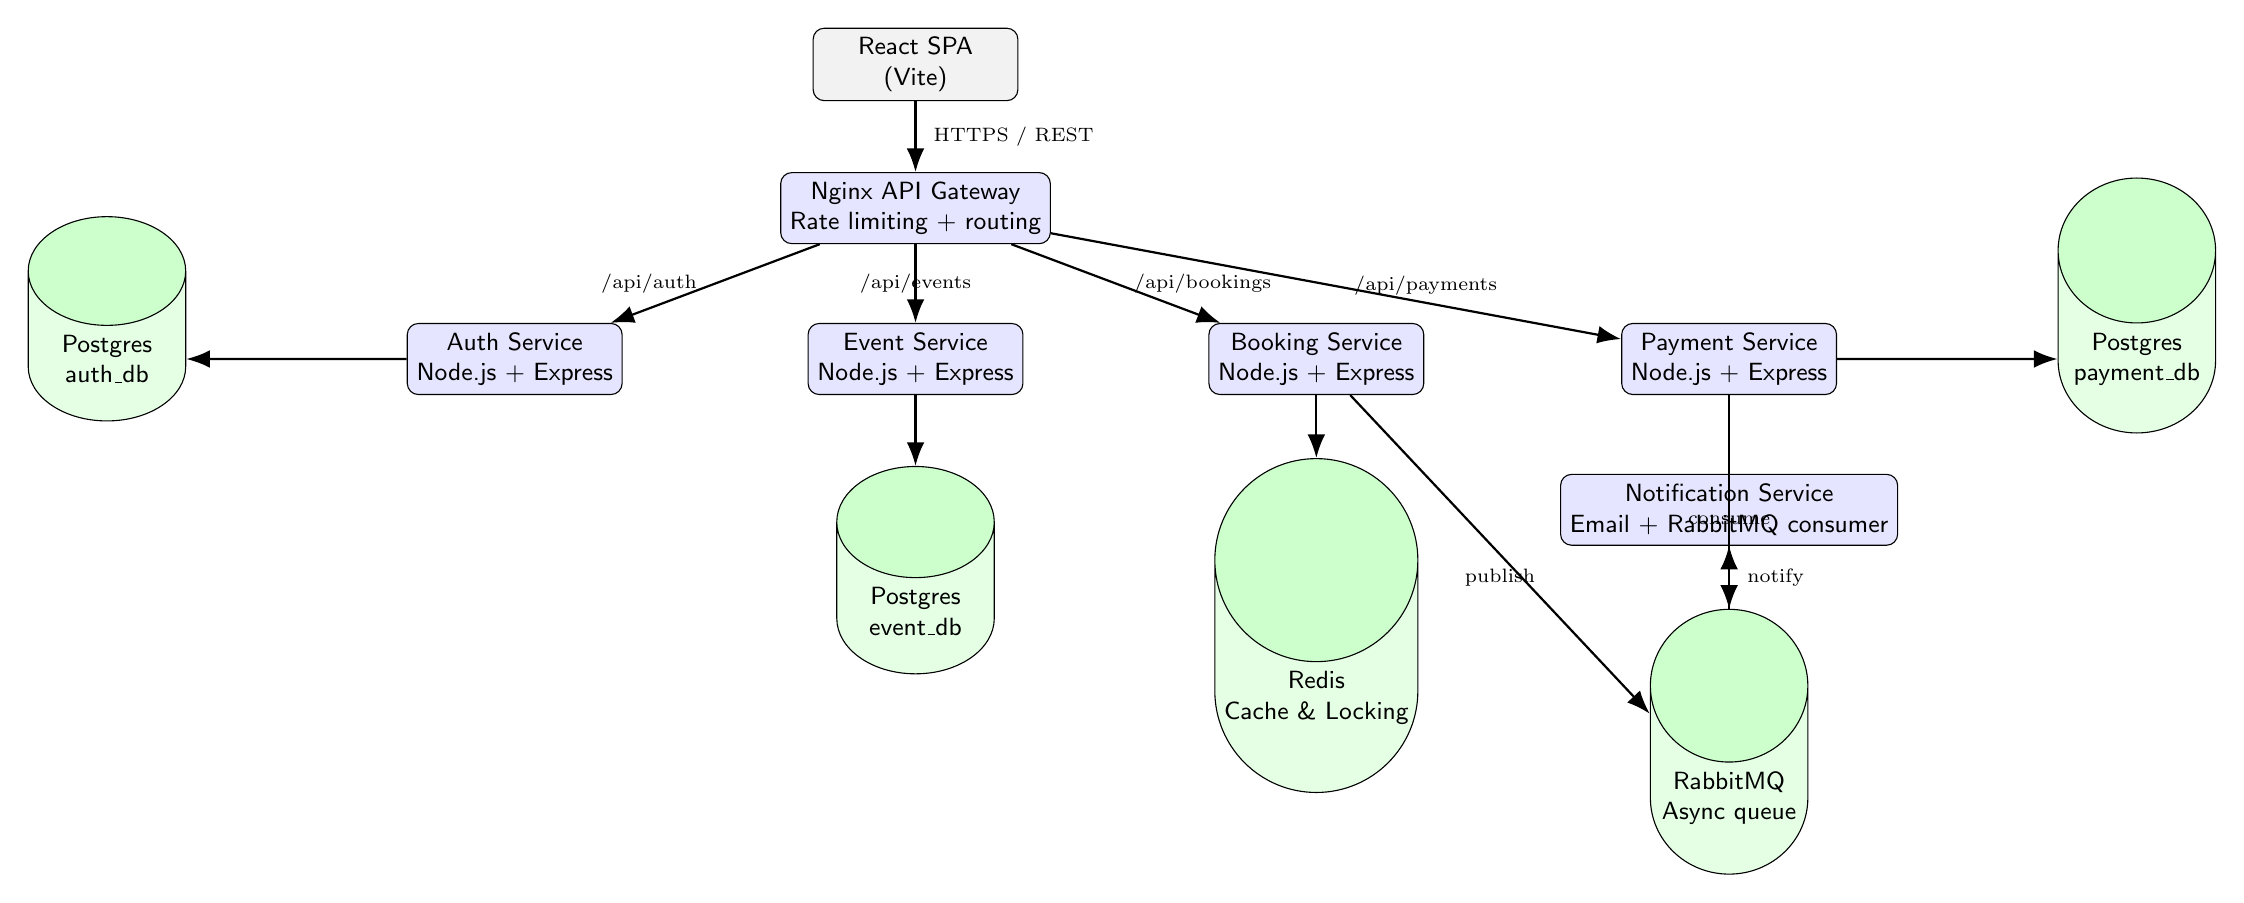
\begin{tikzpicture}[node distance=1.0cm, every node/.style={font=\sffamily\small, align=center}, arrow/.style={-{Latex[length=3mm]}, thick}]
        \tikzstyle{service} = [rectangle, draw=black, rounded corners, fill=blue!10, minimum width=2.4cm, minimum height=0.9cm]
        \tikzstyle{component} = [rectangle, draw=black, rounded corners, fill=gray!10, minimum width=2.6cm, minimum height=0.9cm]
        \tikzstyle{database} = [cylinder, cylinder uses custom fill, cylinder body fill=green!10, cylinder end fill=green!20, shape border rotate=90, draw=black, minimum width=2.0cm, minimum height=0.9cm]
        \tikzstyle{arrowtext} = [font=\scriptsize]

        \node[component] (frontend) {React SPA\\(Vite)};
        \node[service, below=0.9cm of frontend] (gateway) {Nginx API Gateway\\Rate limiting + routing};
        \node[service, below left=1.0cm and 2.0cm of gateway] (auth) {Auth Service\\Node.js + Express};
        \node[service, below=1.0cm of gateway] (event) {Event Service\\Node.js + Express};
        \node[service, below right=1.0cm and 2.0cm of gateway] (booking) {Booking Service\\Node.js + Express};
        \node[service, right=2.5cm of booking] (payment) {Payment Service\\Node.js + Express};
        \node[service, below=1.0cm of payment] (notification) {Notification Service\\Email + RabbitMQ consumer};

        \node[database, left=2.8cm of auth] (authdb) {Postgres\\auth\_db};
        \node[database, below=0.9cm of event] (eventdb) {Postgres\\event\_db};
        \node[database, right=2.8cm of payment] (paydb) {Postgres\\payment\_db};
        \node[database, below=0.8cm of booking] (redis) {Redis\\Cache \& Locking};
        \node[database, below=0.8cm of notification] (rabbit) {RabbitMQ\\Async queue};

        \draw[arrow] (frontend) -- (gateway) node[midway, right=1mm, arrowtext]{HTTPS / REST};
        \draw[arrow] (gateway) -- (auth) node[midway, left=1mm, arrowtext]{/api/auth};
        \draw[arrow] (gateway) -- (event) node[midway, arrowtext]{/api/events};
        \draw[arrow] (gateway) -- (booking) node[midway, right=1mm, arrowtext]{/api/bookings};
        \draw[arrow] (gateway) -- (payment) node[midway, right=1mm, arrowtext]{/api/payments};

        \draw[arrow] (auth) -- (authdb);
        \draw[arrow] (event) -- (eventdb);
        \draw[arrow] (payment) -- (paydb);
        \draw[arrow] (booking) -- (redis);
        \draw[arrow] (booking) -- (rabbit) node[midway, below=0.5mm, arrowtext]{publish};
        \draw[arrow] (payment) -- (rabbit) node[midway, below=0.5mm, arrowtext]{consume};
        \draw[arrow] (rabbit) -- (notification) node[midway, right=1mm, arrowtext]{notify};
    \end{tikzpicture}%
    }
    \caption{Professional architecture diagram for EventSphere, showing synchronous and asynchronous communication.}
    \label{fig:architecture}
\end{figure}

\subsection{Major Components}
\begin{itemize}[itemsep=0.4em]
    \item \textbf{React SPA (Frontend):} A single-page application built with React and Vite, served via Nginx.
    \item \textbf{Nginx API Gateway:} Acts as the entry point for web traffic, handling routing, caching, and rate limiting.
    \item \textbf{Auth Service:} Responsible for registration, login, JWT generation, and profile management.
    \item \textbf{Event Service:} Manages event listing, categories, and detail retrieval.
    \item \textbf{Booking Service:} Handles booking requests with Redis-based locking to prevent double-booking.
    \item \textbf{Payment Service:} Processes payments and triggers asynchronous events.
    \item \textbf{Notification Service:} Sends email notifications using RabbitMQ to decouple the booking flow.
    \item \textbf{PostgreSQL Databases:} Each core service has a dedicated Postgres instance for data isolation.
    \item \textbf{Redis:} Used for caching availability and distributed locking.
    \item \textbf{RabbitMQ:} Provides asynchronous communication and event-driven notification delivery.
\end{itemize}

\subsection{Cloud-Native Principles}
EventSphere demonstrates the following cloud-native principles:
\begin{itemize}[itemsep=0.4em]
    \item \textbf{Scalability:} Services can be scaled independently using Docker Compose or orchestration platforms.
    \item \textbf{High Availability:} Health checks, restart policies, and isolated services reduce the impact of individual failures.
    \item \textbf{Security:} JWT authentication, rate limiting, helmet headers, and password hashing protect the application.
    \item \textbf{Resilience:} Asynchronous RabbitMQ messaging decouples the booking and notification pipelines.
    \item \textbf{Deployment Automation:} Docker Compose provides one-command local deployment with a reproducible environment.
\end{itemize}

\section{Implementation Steps}
This section describes the deployment workflow and key development milestones.

\subsection{Development Setup}
\begin{enumerate}[itemsep=0.5em]
    \item Clone the repository and copy environment variables from \texttt{.env.example}.
    \item Build the frontend with \texttt{npm install} and \texttt{npm run build} inside the \texttt{frontend/} folder.
    \item Start the full stack using \texttt{docker compose up --build -d} from the repository root.
    \item Verify service health using \texttt{docker compose ps} and API health endpoints.
\end{enumerate}

\subsection{Service Deployment}
Each microservice uses a dedicated Dockerfile and runtime configuration:
\begin{itemize}[itemsep=0.4em]
    \item Auth, Event, Booking, Payment services all use Node.js + Express with Sequelize for Postgres.
    \item Notification service runs a lightweight email processor that consumes RabbitMQ events.
    \item Nginx is the gateway and also serves the built React application static files.
\end{itemize}

\subsection{Database and Messaging Setup}
\begin{itemize}[itemsep=0.4em]
    \item PostgreSQL databases are created and initialized using SQL scripts mounted into the containers.
    \item Redis stores booking locks and temporary caching for seat availability.
    \item RabbitMQ manages asynchronous events, ensuring booking success and notification delivery are separate flows.
\end{itemize}

\subsection{Security and Observability}
Security features included in the implementation:
\begin{itemize}[itemsep=0.4em]
    \item JWT authentication and role-based access control.
    \item Helmet.js security headers and CORS restrictions.
    \item Rate limiting at the gateway layer to protect APIs from abuse.
    \item Secure password hashing with bcrypt.
\end{itemize}

\section{Challenges Faced}
The main implementation challenges were:
\begin{itemize}[itemsep=0.4em]
    \item \textbf{Service communication:} Ensuring containers could resolve internal hostnames and that Nginx forwarded requests to the correct backend service.
    \item \textbf{Asynchronous flow:} Designing RabbitMQ messaging so that booking, payment, and notifications remained decoupled without losing transactional consistency.
    \item \textbf{State management:} Preventing double-booking required careful Redis locking and seat availability updates.
    \item \textbf{Deployment reliability:} Configuring Docker Compose health checks and restart policies to ensure services recovered cleanly.
    \item \textbf{Frontend integration:} Connecting the React UI to the API gateway and handling errors gracefully during service outages.
\end{itemize}

\section{Lessons Learned}
Key lessons learned during the project:
\begin{itemize}[itemsep=0.4em]
    \item A microservices architecture improves flexibility, but service orchestration and networking must be carefully designed.
    \item Asynchronous messaging is essential for scalable and resilient workflows in cloud-native systems.
    \item Security must be layered at both the gateway and service levels to protect the full stack.
    \item Docker Compose is an effective deployment tool for development and demonstration, while production systems benefit from Kubernetes or container platform automation.
    \item Clear documentation, including run instructions and architecture diagrams, simplifies handoff and evaluation.
\end{itemize}

\section{Conclusion}
EventSphere successfully demonstrates a realistic cloud-native application using modern deployment practices. The platform supports secure user authentication, event browsing, booking, payment processing, and asynchronous notification delivery. The chosen architecture and implementation align with the assignment goals for scalability, availability, security, and deployment readiness.

\end{document}
